\documentclass[13pt,a4paper]{article}

\usepackage[utf8]{inputenc}
\usepackage{graphicx}
\usepackage{wrapfig}
\usepackage{color}
\usepackage{xcolor}
\usepackage{amsmath}
\usepackage{amssymb}
\usepackage[inkscapelatex=false]{svg}
\usepackage{array, makecell}
\usepackage{mhchem}
\usepackage{tabularx}
\usepackage{svg}
\usepackage{braket}
\usepackage{listings}
\definecolor{commentsColor}{rgb}{0.497495, 0.497587, 0.497464}
\definecolor{keywordsColor}{rgb}{0.000000, 0.000000, 0.635294}
\definecolor{stringColor}{rgb}{0.558215, 0.000000, 0.135316}
\lstset{
    frame=single,
    language=Python,
    basicstyle=\ttfamily\vspace{1em},
}

\usepackage[T1]{fontenc}
\usepackage[utf8]{inputenc}
\usepackage[lf]{Baskervaldx} % lining figures
\usepackage[bigdelims,vvarbb]{newtxmath} % math italic letters from nimbus Roman
\usepackage[cal=boondoxo]{mathalfa} % mathcal from STIX, unslanted a bit
\renewcommand*\oldstylenums[1]{\textosf{#1}}

\usepackage{multicol}
\usepackage{colortbl}
\usepackage[Export]{adjustbox}
\adjustboxset{max size={0.9\linewidth}{0.9\paperheight}}
\usepackage[colorlinks=true,linkcolor=red,citecolor=green]{hyperref}

\textwidth=16cm
\textheight=23cm
\topmargin=-2cm
\oddsidemargin=0cm
\setlength{\parindent}{0em}
\setlength{\parskip}{0.6em}
\setlength{\jot}{12pt}
\renewcommand{\arraystretch}{1.4}
\renewcommand{\theadfont}{\bfseries}
\newcommand{\todo}[1]{\textcolor{red}{TODO: #1}}


\begin{document}
\title{
    \LARGE
    \textbf{SATFD lab 04}
}
\author{
    \large
    Dawid Karpiński, 25.04.2024 r.
}
\date{}
\maketitle

\section{Noisy sine signal}
\subsection{FIR filters}

\begin{figure}[ht!]
    \centering
    % \caption{\textbf{FIR Highpass filter}}
    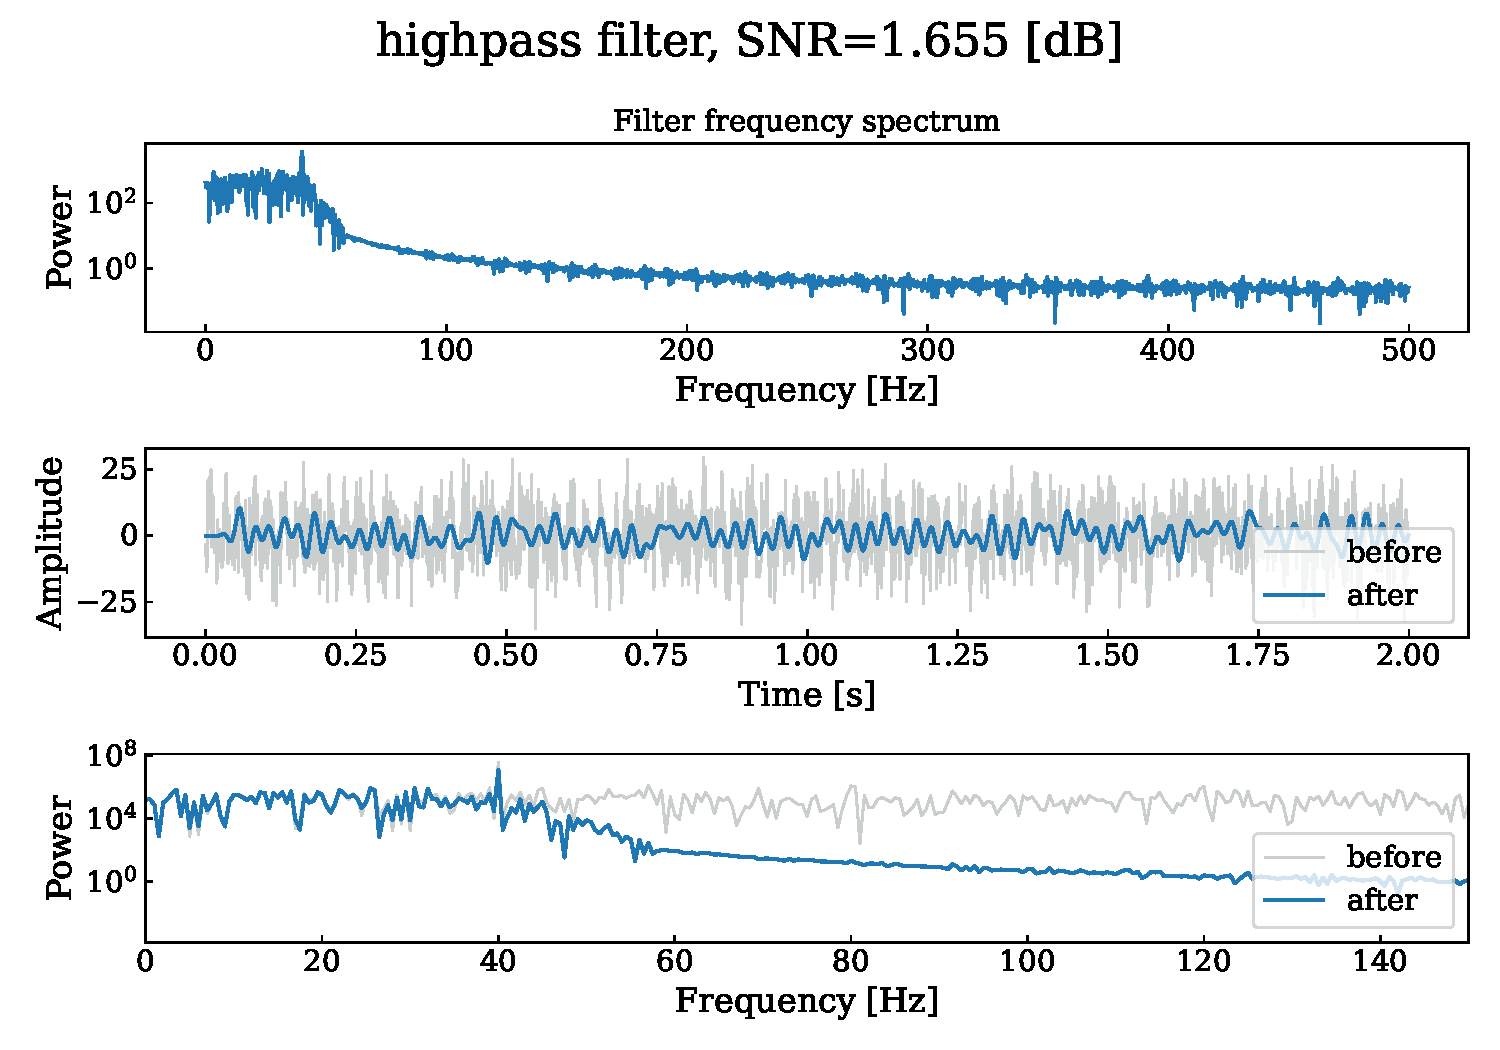
\includegraphics[width=0.9\linewidth]{fir.highpass.pdf}
\end{figure}
\pagebreak

\begin{figure}[ht!]
    \centering
    % \caption{\textbf{FIR Highpass filter}}
    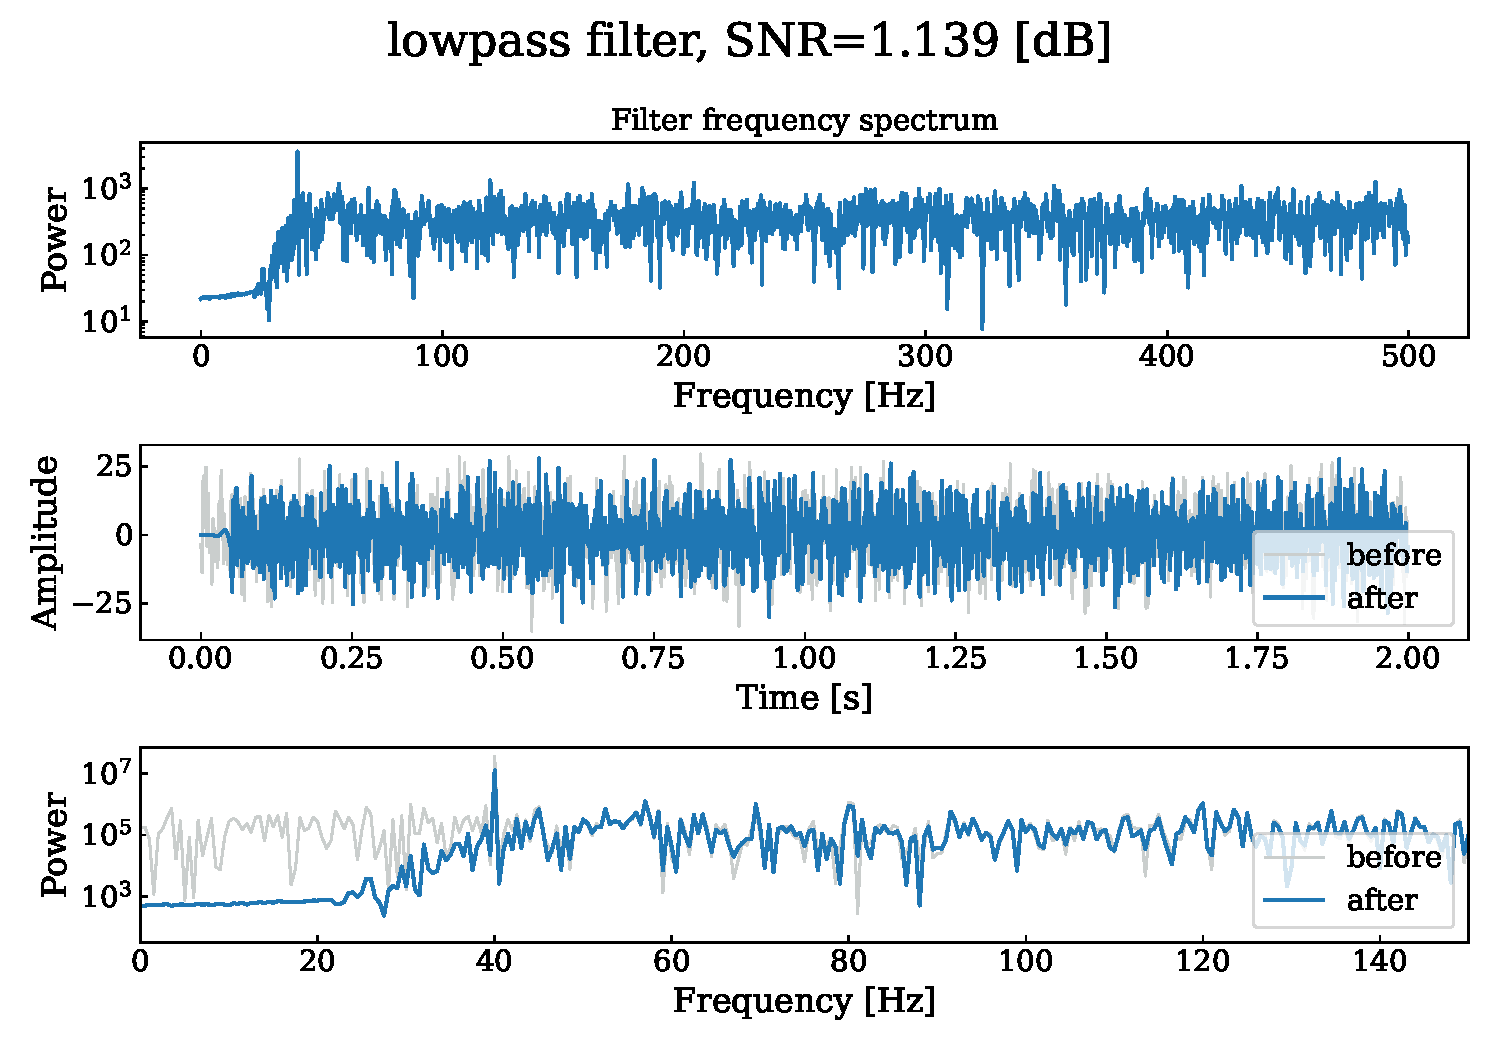
\includegraphics[width=0.9\linewidth]{fir.lowpass.pdf}
\end{figure}

\begin{figure}[ht!]
    \centering
    % \caption{\textbf{FIR Highpass filter}}
    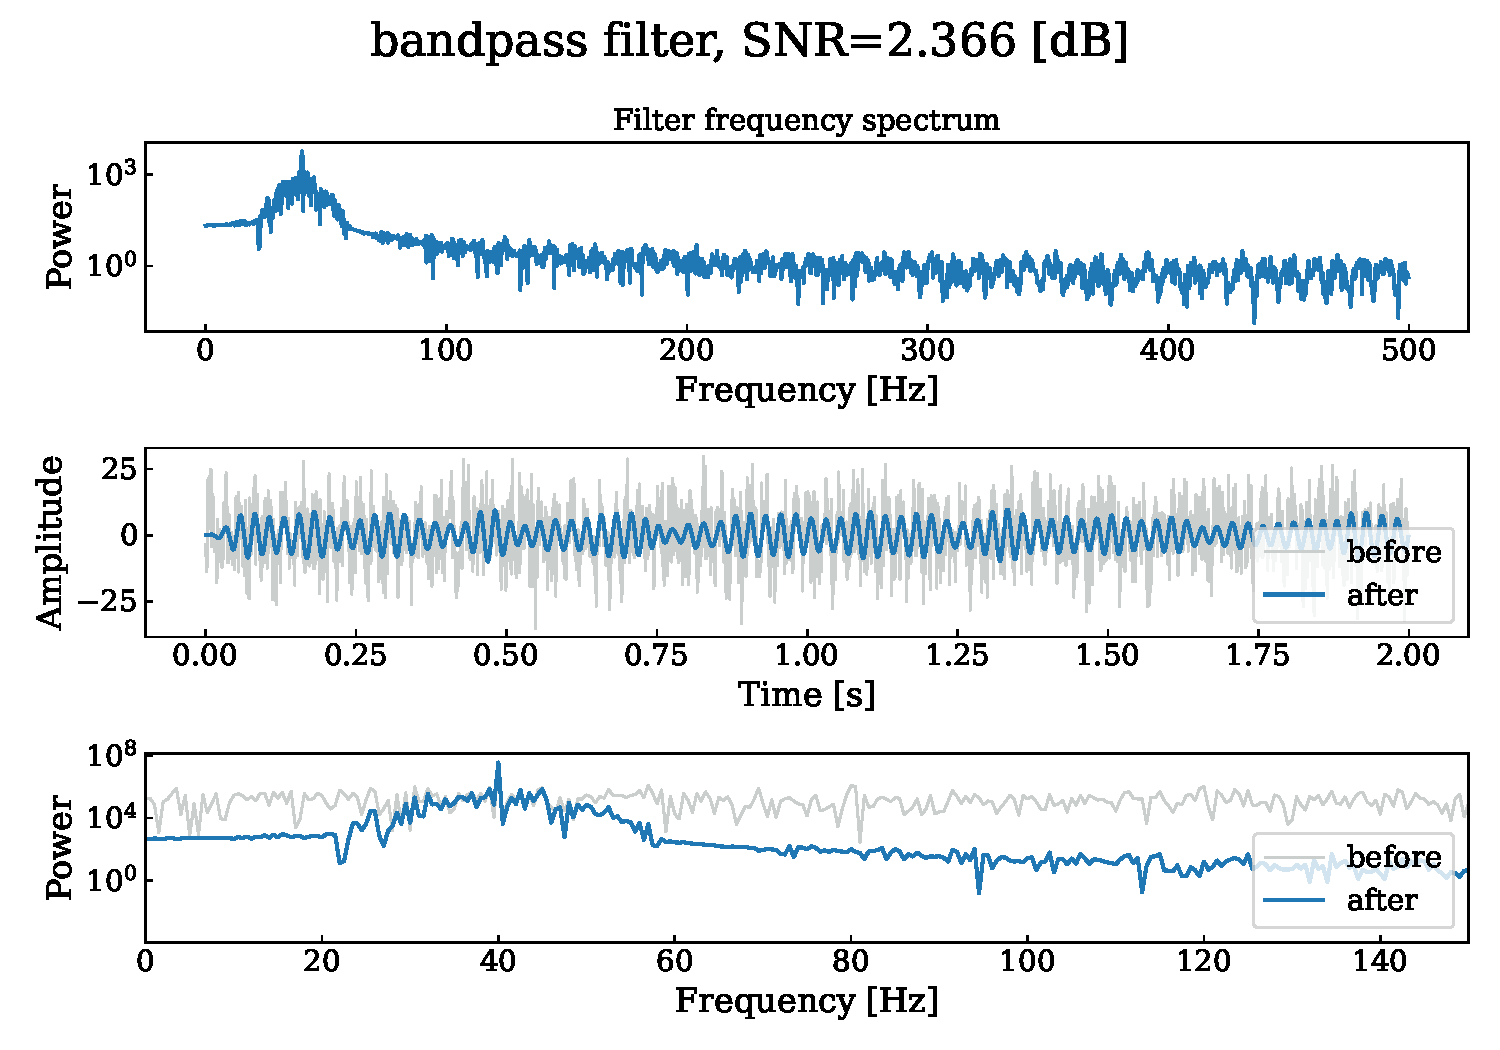
\includegraphics[width=0.9\linewidth]{fir.bandpass.pdf}
\end{figure}
\pagebreak


\subsection{IIR filters}

\begin{figure}[ht!]
    \centering
    % \caption{\textbf{FIR Highpass filter}}
    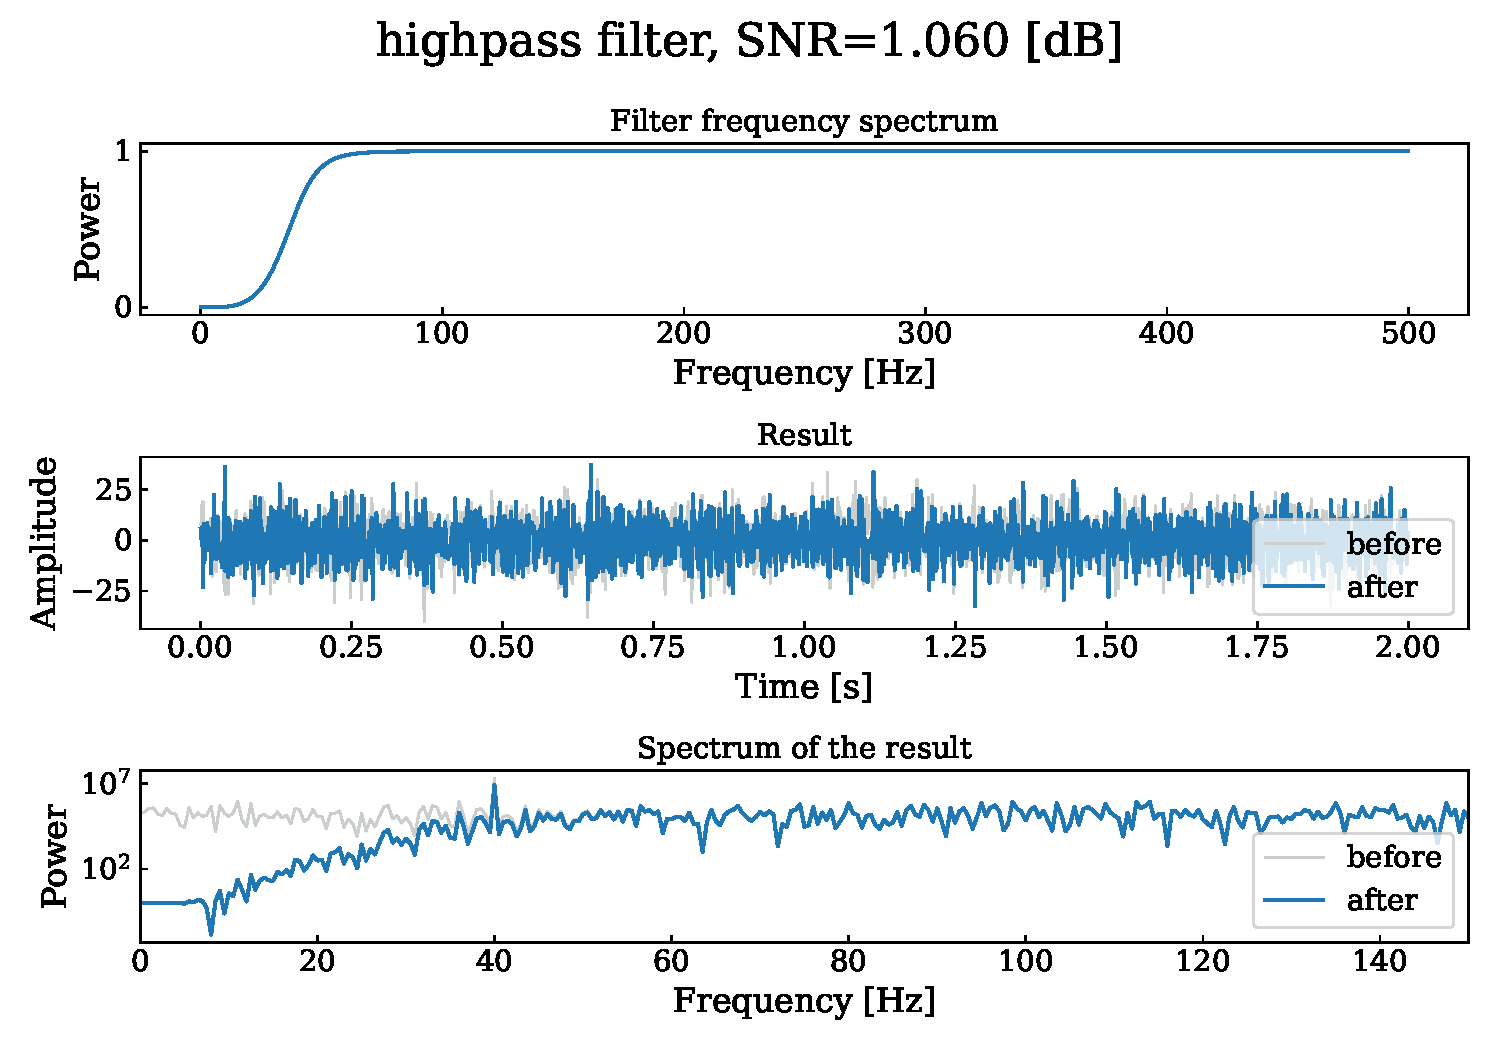
\includegraphics[width=0.9\linewidth]{iir.highpass.pdf}
\end{figure}

\begin{figure}[ht!]
    \centering
    % \caption{\textbf{iir Highpass filter}}
    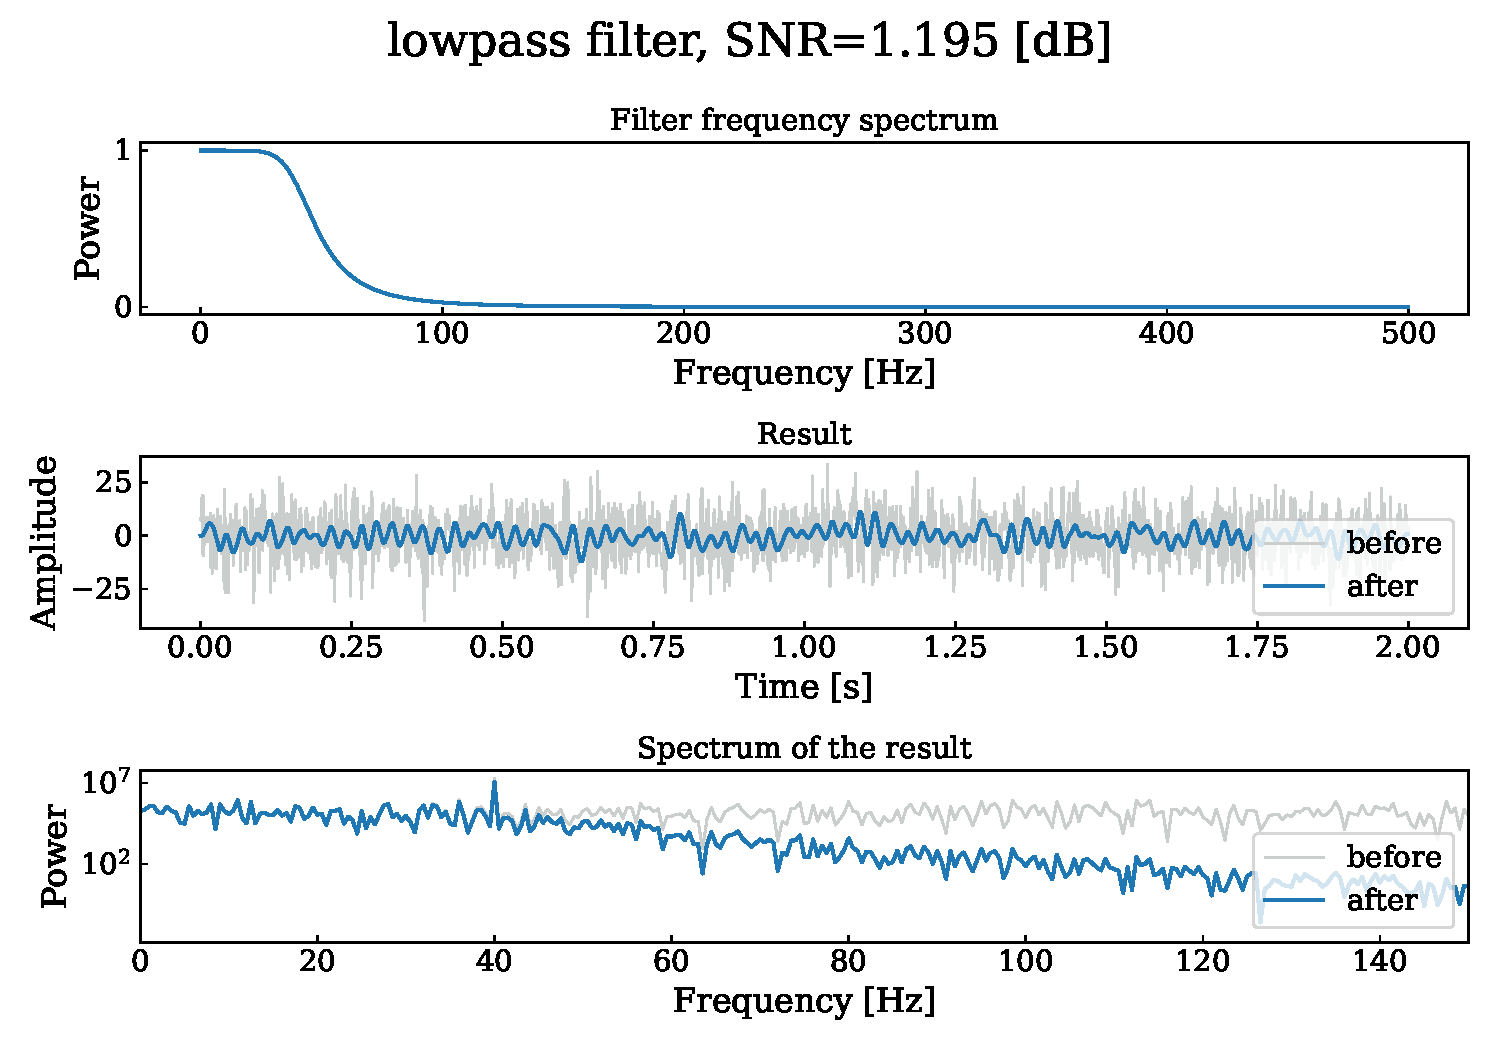
\includegraphics[width=0.9\linewidth]{iir.lowpass.pdf}
\end{figure}

\begin{figure}[ht!]
    \centering
    % \caption{\textbf{iir Highpass filter}}
    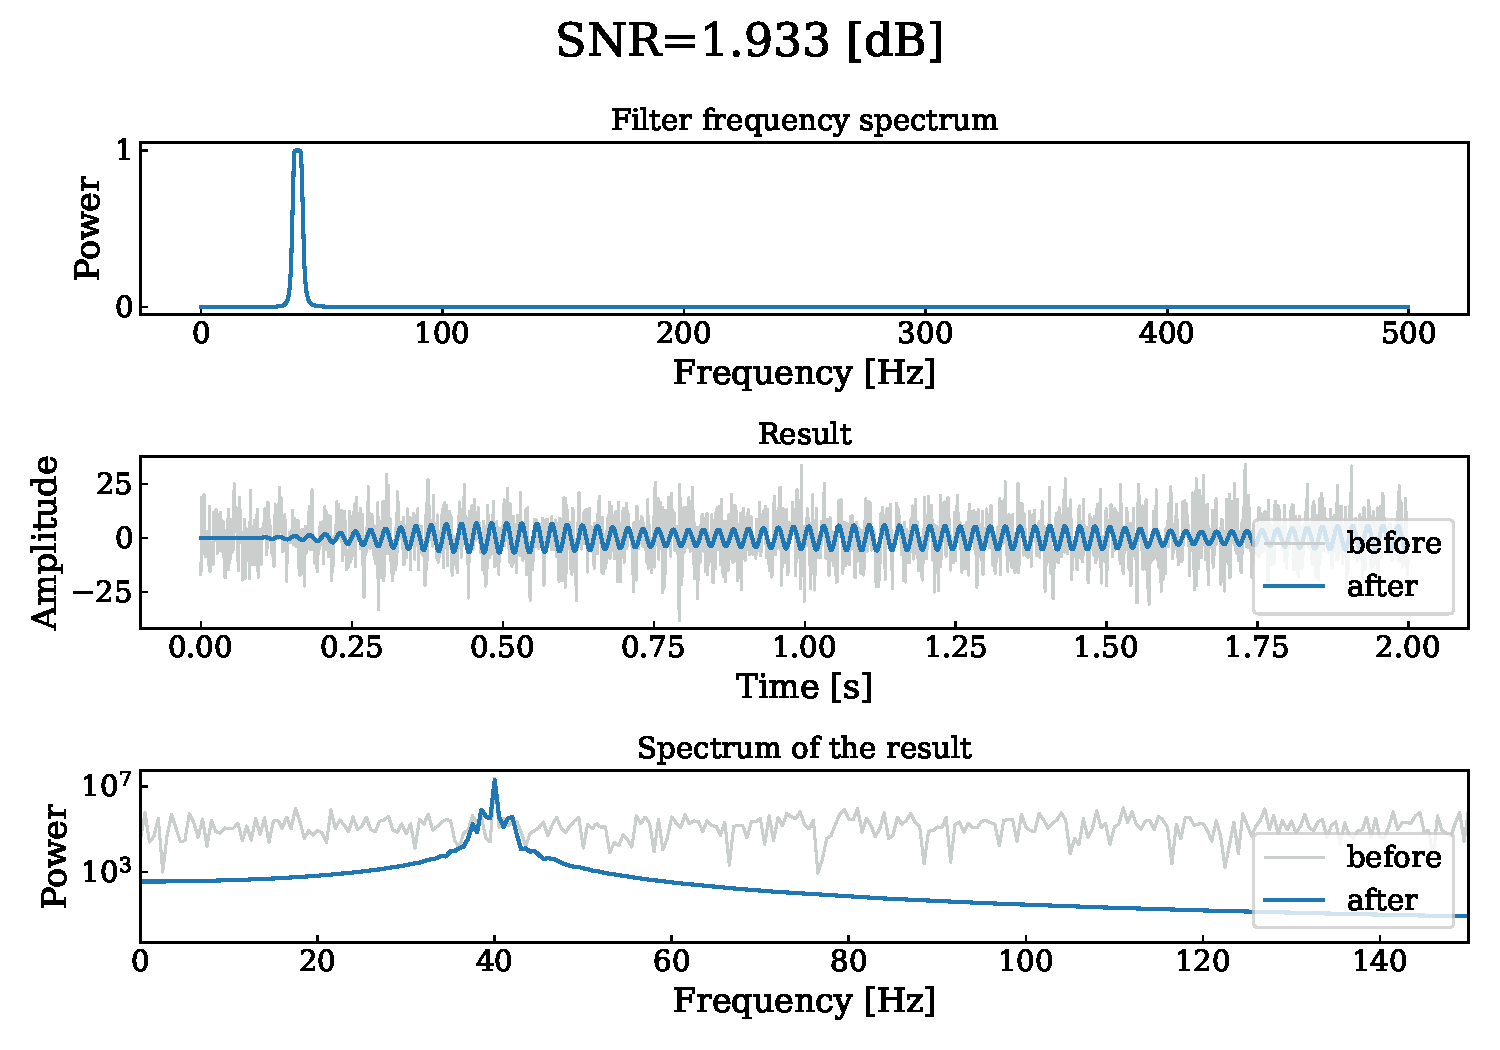
\includegraphics[width=0.9\linewidth]{iir.bandpass.pdf}
\end{figure}


\section{Two sine waves}

\begin{figure}[ht!]
    \centering
    \caption{\textbf{Sum of two sine waves}}
    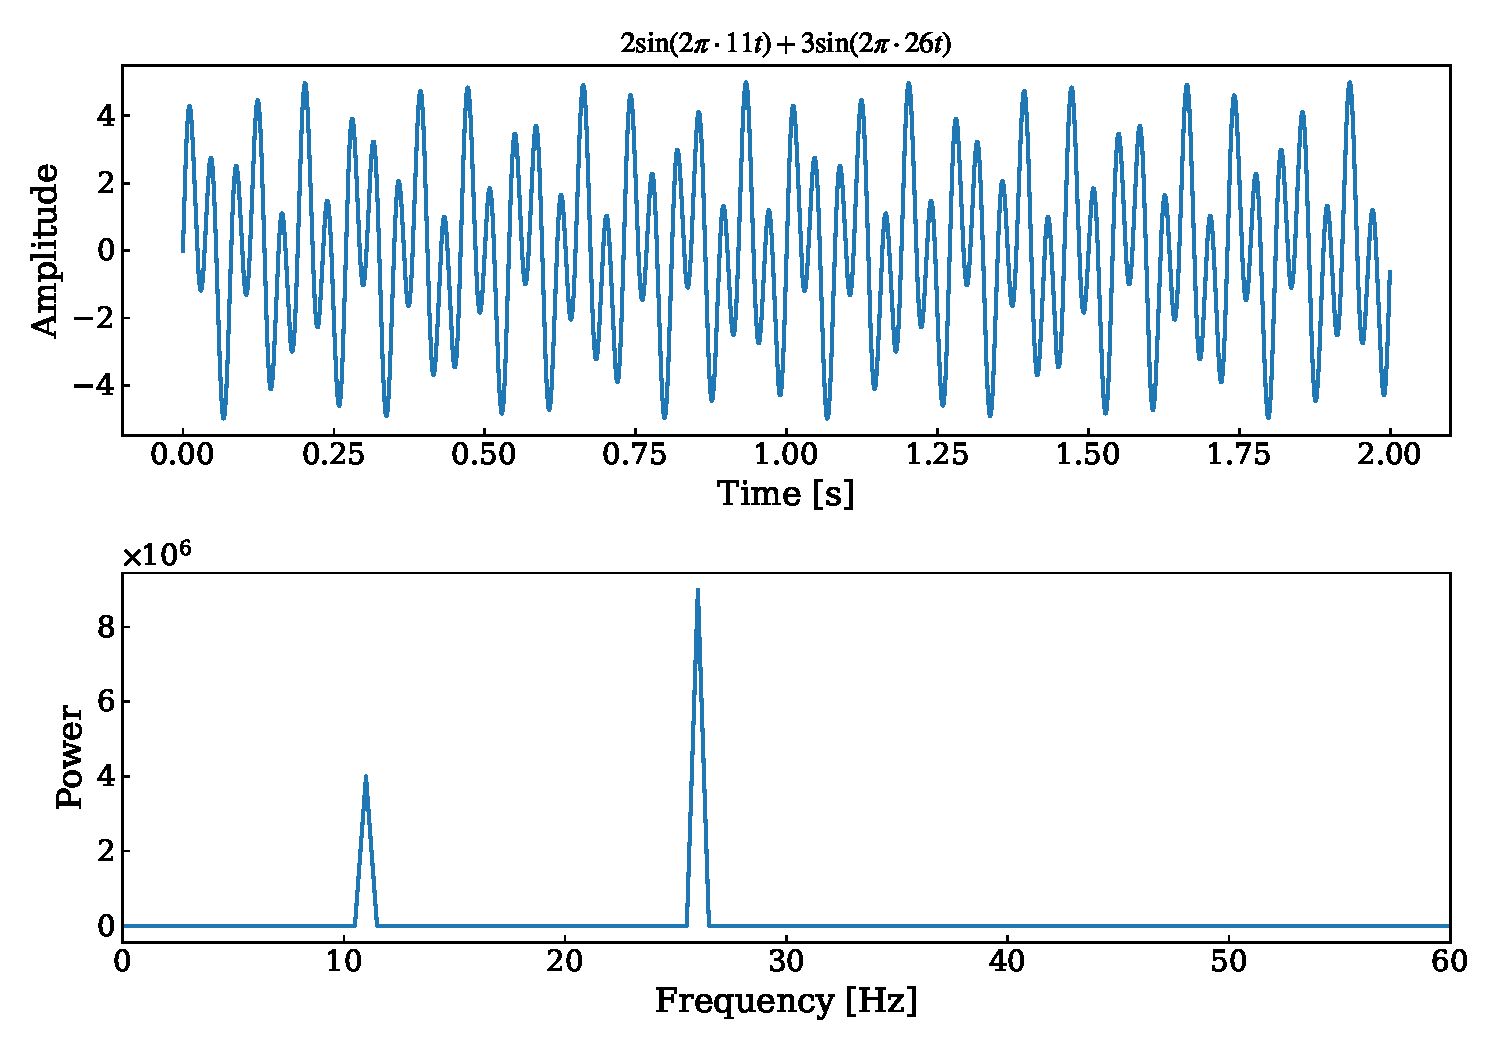
\includegraphics[width=0.9\linewidth]{two_sin.pdf}
\end{figure}

\begin{figure}[ht!]
    \centering
    \caption{\textbf{Result after highpass filter of two sines}}
    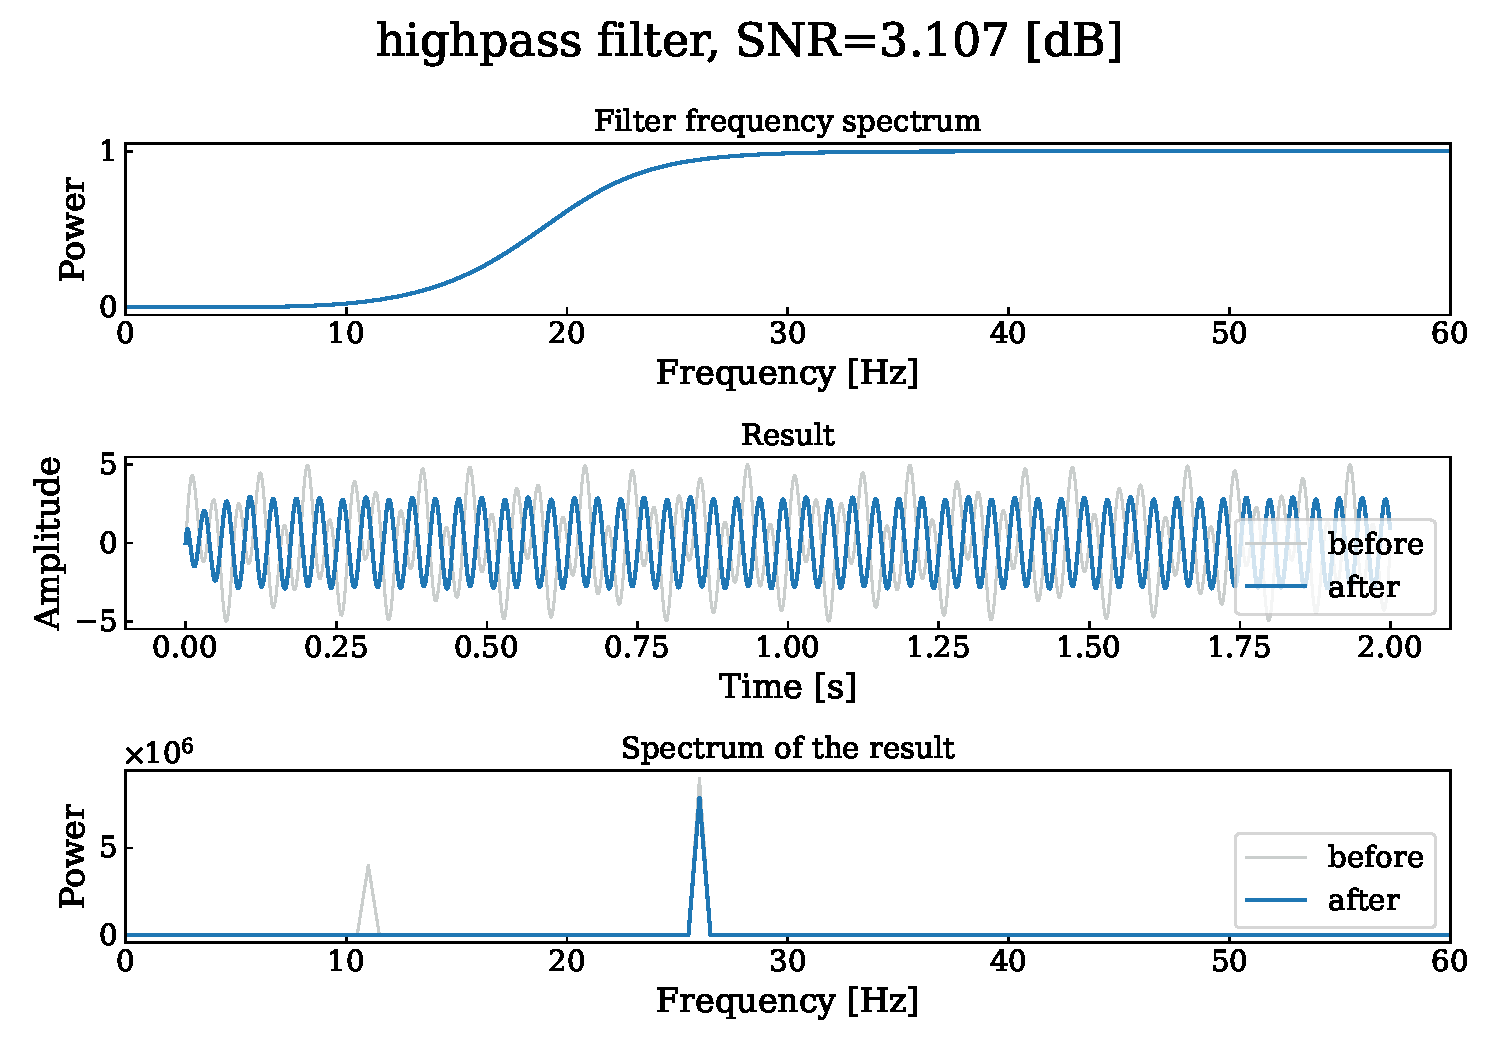
\includegraphics[width=0.9\linewidth]{filter_two_sin.highpass.pdf}
\end{figure}

\begin{figure}[ht!]
    \centering
    \caption{\textbf{Result after lowpass filter of two sines}}
    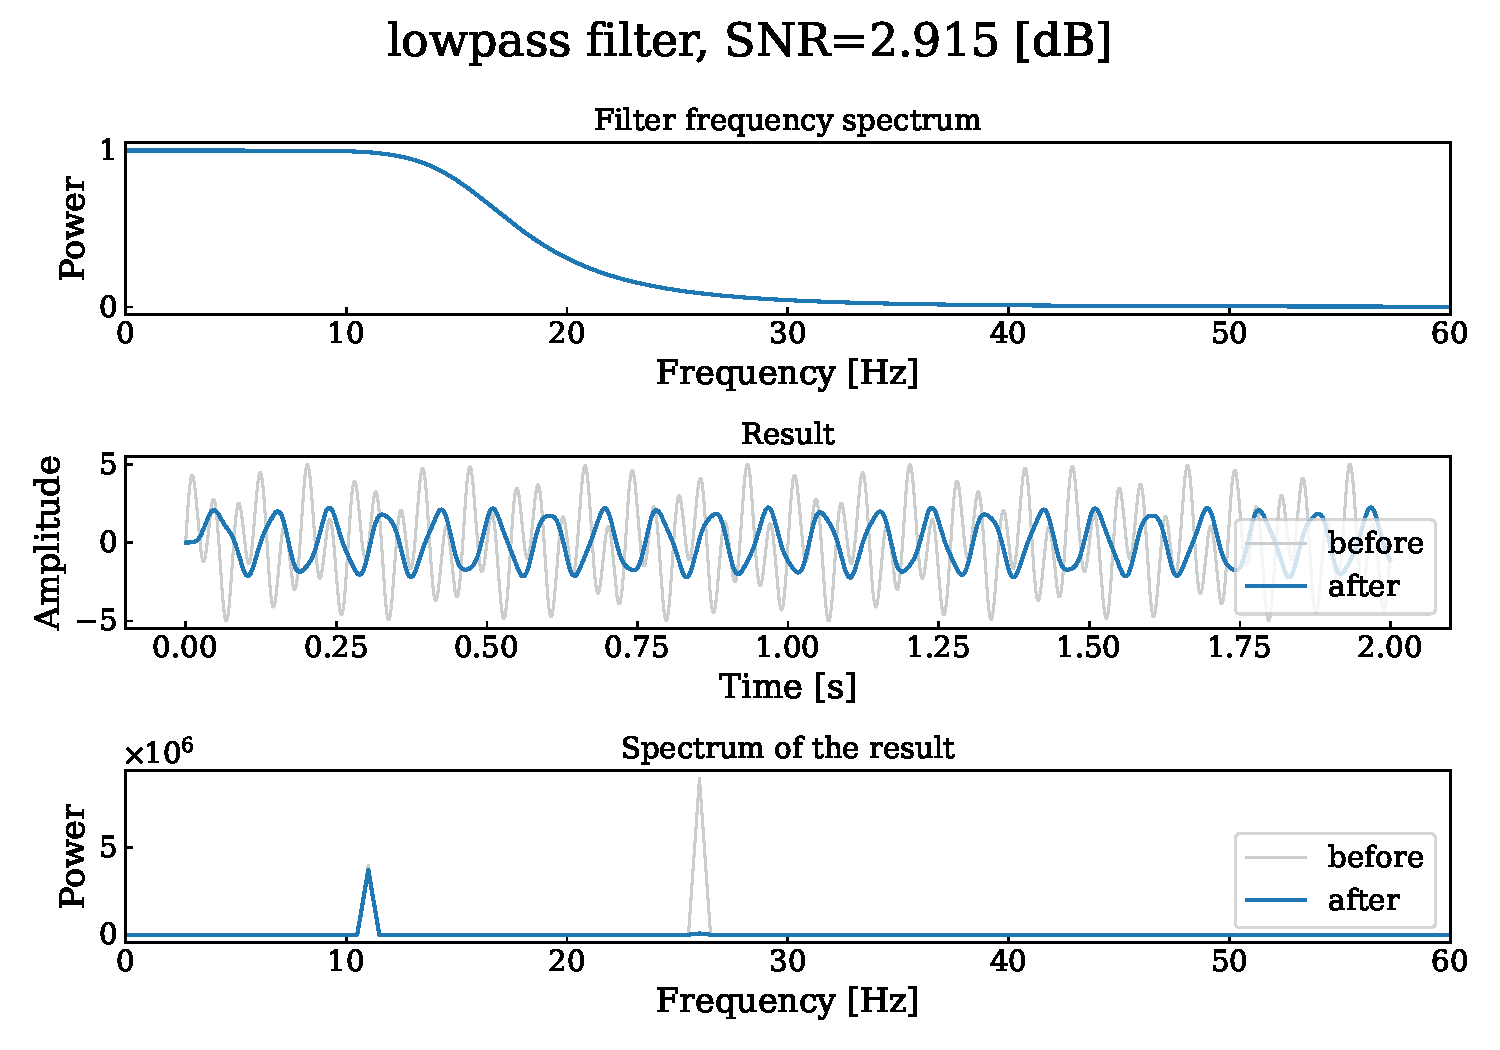
\includegraphics[width=0.9\linewidth]{filter_two_sin.lowpass.pdf}
\end{figure}

\section{Noisy ECG signal}

\begin{figure}[ht!]
    \centering
    \caption{\textbf{ECG before and after applying the filter}}
    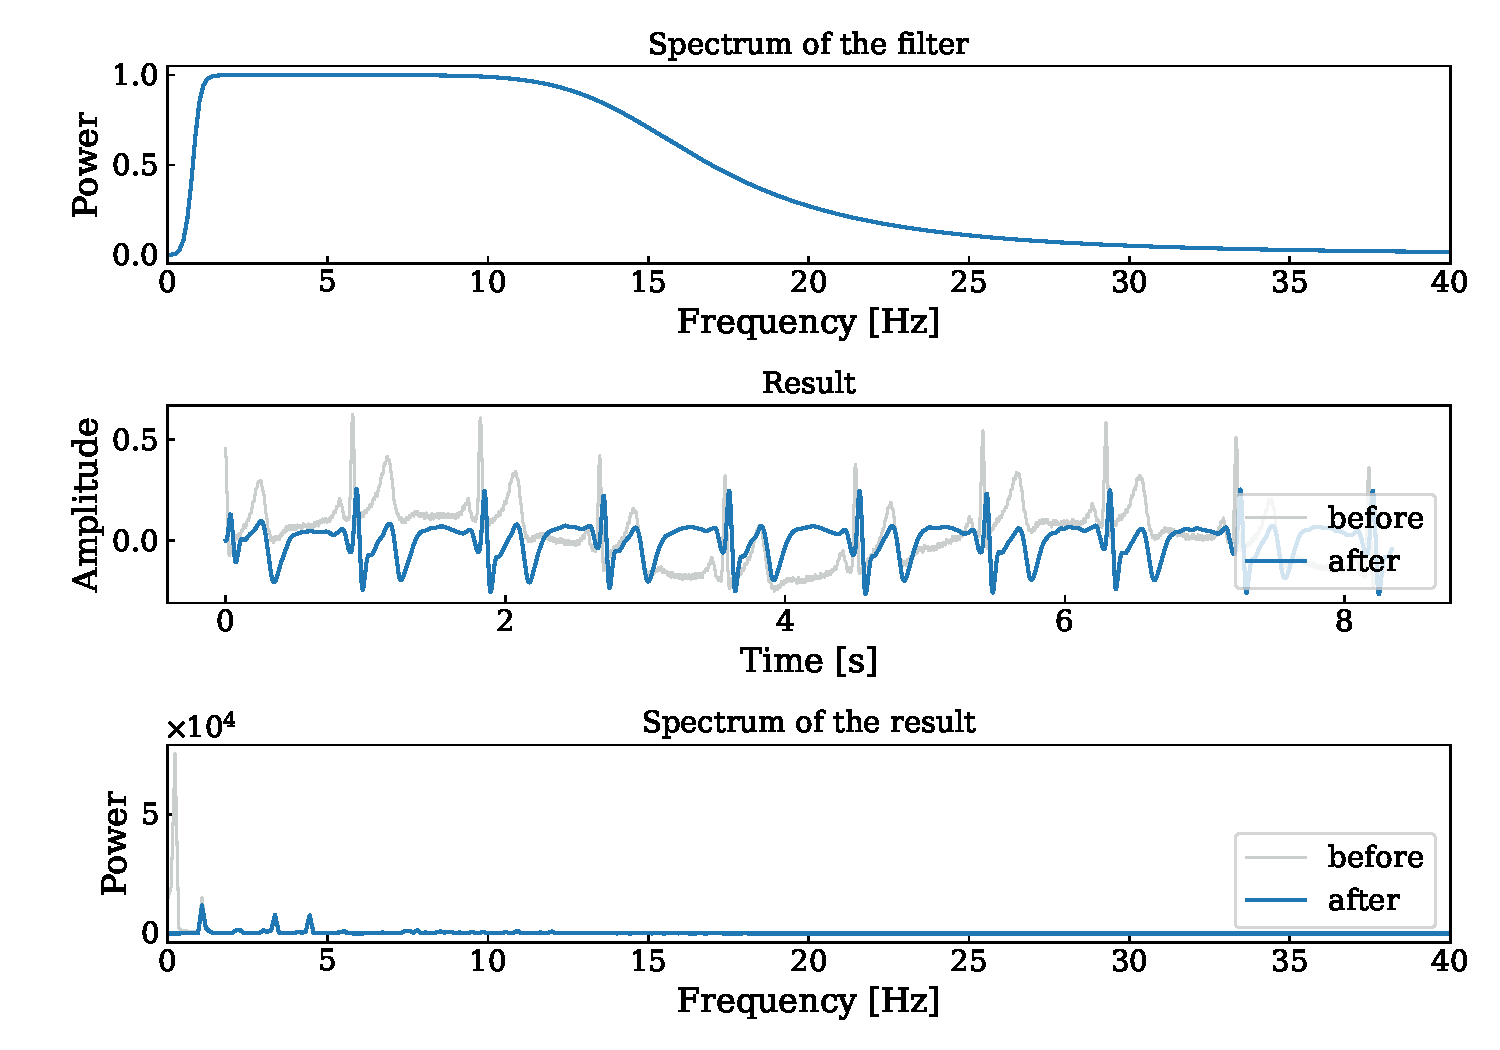
\includegraphics[width=0.9\linewidth]{./ecg_filter.pdf}
\end{figure}

\section{Conclusion}

The entire code for generating the data and plots can be found at:

\url{https://github.com/davkk/signal-analysis/tree/main/sat/lab04}

\end{document}
